\documentclass[sigconf]{acmart}

\usepackage{graphicx}
\usepackage{hyperref}
\usepackage{todonotes}

\usepackage{endfloat}
\renewcommand{\efloatseparator}{\mbox{}} % no new page between figures

\usepackage{booktabs} % For formal tables

\settopmatter{printacmref=false} % Removes citation information below abstract
\renewcommand\footnotetextcopyrightpermission[1]{} % removes footnote with conference information in first column
\pagestyle{plain} % removes running headers

\newcommand{\TODO}[1]{\todo[inline]{#1}}

\begin{document}
\title{Big Data = Big Bias? An Analysis of Google Search Suggestions}

\author{Gabriel Jones}
\affiliation{%
  \institution{Indiana University Bloomington}
  \city{Bloomington} 
  \state{Indiana} 
  \country{USA}
}
\email{gabejone@indiana.edu}

\author{Mathew Millard}
\affiliation{%
  \institution{Indiana University Bloomington}
  \city{Bloomington} 
  \state{Indiana} 
  \country{USA}
}
\email{mdmillar@indiana.edu}

\renewcommand{\shortauthors}{M. Millard}

\begin{abstract}
Since its origins, Big Data has promised to revolutionize the world. Scholars have wisely noted that it represents a paradigmatic shift from conventional norms of data, but the public has latched onto provocative but unrealistic narratives that deify Big Data as omniscient, infallible, and impervious to bias. Confiding in such narratives diminishes the integrity of credible science and poses serious ethical challenges, but these challenges are more likely overlooked because the problematic narratives seem to reject the need for ethical discussion. The authors argue that such blind optimism will cause irreversible damage to society if left unchecked. First, we debunk the fallacious narratives people tend to tell about Big Data, offering a more realistic discussion of its merits and its limitations. We then explore how analytical or algorithmic bias and sampling bias, two problems that statisticians have faced since long before the onset of Big Data, present pitfalls for deriving knowledge from data. We examine how the ethical implications of these pitfalls can cause serious damage in society. We conclude that effective, credible, and ethically sound Big Data analysis must obey the principles of transparency, clear and appropriate objective definition, and self-correcting feedback mechanisms.
\end{abstract}

\keywords{i523, hid104, hid226, Big Data, Ethics, Algorithmic Bias, Sample Bias}

\maketitle

\section{Introduction: Fallacious Narratives about Big Data}

In 2008, {\em Wired.com's} Chris Anderson wrote an article that captures the general optimism with which people conceptualize Big Data. The article, with its self-explanatory title ``The End of Theory: The Data Deluge Makes the Scientific Method Obsolete'', argues that Big Data provides such a complete, infallible view into reality that we no longer need conventional methods of scientific inquiry but need only to look at what the data tell us. According to Anderson, ``With enough data, the numbers speak for themselves''\cite{Anderson2008}. This fervorous optimism was further extended in a 2013 book by Mayer-Schonberger and Cukier titled {\em Big Data} where authors assert that Big Data is synonymous with all data. In the past, researchers could only look at samples of data with limited scope, but Big Data, the authors claim, represents not a sample but a complete set\cite{Lagoze2014}. A dataset of Twitter posts is viewed as synonymous with a complete, unbiased set of all of society's thoughts. By analyzing such a dataset, they conclude that they can confidently answer any question about how all of society thinks and behaves\cite{Harford2014}.

Cheerleaders for Big Data, such as Anderson, Mayer-Schonberger, and Cukier to make five exciting but yet flatly incorrect claims: that bigger is always better; that data analysis produces indisputably accurate results; that every data point can be studied, eliminating the need for archaic statistical sampling techniques; that studying causation is no longer needed since correlational patterns tell us all we need to know; and that scientific and statistical models are obsolete, since Big Data is itself sufficient. They have tended to extrapolate from the early success of the Google Flu Trends which at the time successfully embodied such grandiose, idealistic views. The Google Flu Trends project employed a theory-free set of algorithms that studied search engine results to predict flu outbreaks faster and more accurately than the Center for Disease Control. Allowing the numbers to ``speak for themselves'', Google determined that the number of searches about the Flu were correlated with flu outbreaks, so they concluded that more searches could accurately predict a greater spread\cite{Harford2014}. 

At first it worked brilliantly. But in February 2013, just a month before the {\em n = all} proposition was published in {\em Big Data}, it made headlines for failing miserably, overestimating actual trends in 2013 by over 140 percent, leading Google to humbly terminate the program. The overconfidence of such an enormous dataset, viewed as a complete representation of reality free of gaps or inconsistencies, blinded them to its inherent flaws. For one, searches involving the term {\em influenza} are hardly an unbiased determinant of flu prevalence. They committed a classic statistical mistake by failing to consider confounding variables: the other reasons why people might search for the word {\em influenza}. Rather than adapting their model to fit changing patterns in the data, they assumed that the numbers could speak for themselves\cite{Harford2014}. 

But blind proponents of Big Data bury the Google Flu Trends fiasco as just one not particularly convincing counterexample, giving superficial explanations that do not challenge Big Data's position as an infallible deity. In reality, such failure is the rule rather than the exception. Even Gartner, a company publicly known for pushing the importance of Big Data, estimated that 60 percent of Big Data projects would fail\cite{Gartner2015}. But it's not just a matter of occasional success or failure; many people in all disciplines misunderstand the nature of Big Data and therefore have unrealistic expectations. The narrative of the Target coupon case shows that society still regards the potential of Big Data as omniscient even if its execution is occasionally flawed. The story is narrated somewhat as follows.

In 2012, Target had collected enough purchasing data about pregnant women that they determined a particular high school girl was pregnant. When coupons for baby care items mixed in with general coupons started showing up in the mail, the father angrily visited the store manager to complain, suggesting that the store was encouraging teen pregnancy. The manager understood his frustration and called twice to apologize, but on the second call, the father's mood was different. The father offered his own apology because Target was right. His daughter was pregnant, and Target's Big Data analytics managed to discover this before him\cite{Duhigg2012}.

While such a rose-colored narration fits well within the aforementioned grandiose conceptions of Big Data, a closer look shows that this successful case is overblown. While the anecdote seems to prove that Target's algorithms are infallibly accurate -- that everyone receiving baby care coupons is pregnant -- this is very unlikely. While the popular account suggests that Target mixes in coupons targeted towards pregnant women with other coupons to avoid spooking such women about their algorithmic accuracy, a much more credible explanation is that many women see mixed advertisements precisely because Target is unsure which ones actually are pregnant\cite{Harford2014}. Even women who Target does suspect are pregnant have shopping interests outside of baby care items. While the algorithms help not to waste money by sending the coupons to, say, a single male adult living alone, they hardly indicate any reliable accuracy of pregnancy prediction. Of course, this is an empirical question that could be answered by researching how often pregnancy-targeted ads are sent to pregnant women versus those who aren't. But without having a methodologically sound study prove consistent accuracy, it's unwise to extrapolate from the anecdote and assume that Big Data done right is omniscient.

Critiquing the dominant reading of the Target case is not meant to suggest that Big Data has no value. Afterall, Target likely improved the efficiency of targeted advertising through Big Data by more accurately segmenting those who {\em might} be pregnant. But the important thing to keep in mind is that ultimately, models of the world and the data that feed them are imperfect. Models reflect the biases of those who create them, and data reflect biases inherent in sampling methods, time periods, and society in general. Cathy O'Neal, a former professor and Wall Street algorithm specialist with a mathematics degree from Harvard, observes that any model of the world ``begins with a hunch, an instinct about a deeper logic beneath the surface of things''\cite{Wharton2016}. Human potential for bias and faulty assumptions can creep in. Of course, hunches or working thesis provide a necessary part of the scientific method of inquiry. Human intuition can be useful, as long there exist mechanisms by which those hunches can be evaluated and revised when necessary\cite{Wharton2016}.

Perhaps the most common example of successfully wielding insightful models is depicted by the movie {\em Moneyball}, based on a true story. Oakland A's General Manager Billy Beane hypothesized that conventional performance metrics were overrated whereas more obscure measures better predicted overall success. He worked with statistician Bill James to create models that helped Beane decide which players to acquire and which to let go. The once obscure method has become a staple of baseball analytics. According to O'Neal, the model works for three main reasons: it allows for transparent analysis; its objectives are clear and appropriately quantifiable; and it includes a self-correcting feedback mechanism of new inputs and outputs, allowing it to be honed and refined. Models go wrong when they lack these three healthy attributes: ``the calculations are opaque; the objectives attempt to quantify that which perhaps should not be; and feedback loops, far from being self-correcting, serve only to reinforce faulty assumptions''\cite{Wharton2016}.

But models are only one factor in determining the efficacy of Big Data analysis. Since the very nature of data analysis is to extrapolate from limited samples, not only must researchers realize that models include human bias, but data itself is imperfect. It's true that data never lie. But it's false to assume they tell the truth. Data by themselves don't say anything; they simply are\cite{Crawford2013}. No matter how large and complex a dataset, it is always up to researchers to interpret the data to make meaningful claims. This is the essence of the scientific method that some want to reject.

\section{Algorithmic and Sample Bias: The Threats that Never Disappeared}

Humans, as imperfect beings, should never assume that our creations are without flaw and bias. In many ways, mistakes and flawed thinking can trickle into the processes we come up with. This is the idea behind the fallibility of models created by humans with respect to algorithms used for handling Big Data. Some algorithms come with biases based on narrow thinking with a broad scope to cover. Other biases come from the assumption that the Big Data set being used is representative of the population when it really isn't. In any scenario, the creator is prone to introducing bias into any given algorithm, which can make it difficult to trust the results that the algorithm produces. With this in mind and considering the importance of specific findings, there is a lot at stake here. In some cases, lives can be changed for better or worse.

Sometimes algorithms, as models laden with the biases of their creators, can unintentionally manipulate readings of data in ways that reinforce false positives. But not all algorithms are wrong. In fact, machine learning shows us that often a well-written algorithm fed with good data can outperform human knowledge on everything from chess to medical diagnosis. But there's a problem with Big Data; it's inherently messy, complex, and distorted. Contrary to popular opinion that views it as a perfect representation of reality -- recall the {\em n = all} proposition -- Big Data is a black box where typical issues with data quality hide themselves rather than disappearing. No matter how large or complex the dataset, the old adage still remains true: garbage in, garbage out. 

{\em The Literary Digest} experienced the concept of garbage in, garbage out firsthand during the 1936 US presidential election, which pitted the Republican Alfred Landon against the wildly popular democrat Franklin D. Roosevelt. Roosevelt was particularly popular among the working class, the US majority, whereas Landon resonated well with the upper middle class and elites\cite{Harford2014}. {\em The Literary Digest} Tried to predict the outcome of the election by sending out surveys to its own subscribers and by looking people up in phone and automobile registries. During the great depression, the people that owned phones, cars, and subscribed to the  {\em The Literary Digest} tended to be more affluent and republican. After sending out 10 million ballots and receiving back nearly a fifth of them, they predicted that Alfred Landon would win with an astonishing 57 percent of the popular vote. They could not have been more wrong. Landon earned less than 40 percent of the popular vote, losing by a landslide\cite{Crossen2006}. This case has become the archetype example that data from a bias sample will lead to bias results. Increasing the volume of bad data only succeeds in producing a very precise incorrect conclusion, creating a false sense of confidence in something inherently wrong.

Although the {\em The Literary Digest} used lots of data, by definition their sample did not involve Big Data\cite{Lagoze2014}. But if we reject the {\em n = all} proposition, we can see that Big Data is still a sample and is therefore potentially vulnerable to sample bias. But while any statistically literate person can understand what went wrong with {\em The Literary Digest}, sample bias with Big Data is much more complicated and difficult to identify. For many people, random samples of social media data appear impervious to sample bias. Researchers conducting Twitter sentiment analyses often claim objectivity in representing the real world accurately, concluding that patterns observed in these vast, complex webs occur the same way offline. Despite the conflation of people and Twitter users, the two are not synonymous. Twitter users are by no means representative of the population. A Pew Research project in 2013 found that US-based Twitter users ``were disproportionately young, urban or suburban, and black''\cite{Boyd-Crawford2011}. To complicate things further, we cannot assume that Twitter data accurately represent how users behave because users and accounts are not a one-to-one relationship. Some accounts have multiple users, and some users own multiple accounts. Some accounts are just bots that automatically produce content, and some accounts are created and forgotten, going years without use. Furthermore, among active accounts, data are skewed by how some accounts dominate the discourse. Whereas some users post multiple times per day, others use the site only to view content. In fact, 40 percent of active users view content without making contributions, according to 2011 data from Twitter Inc\cite{Boyd-Crawford2011}. The notions of what it means to be active, to participate, and to be a user require critical examination that's almost universally lacking.

The aforementioned examples highlight problems with available Twitter data, but there's also a problem with the integrity of available data. Twitter only makes a fraction of its data publicly available through its APIs. The supposed firehose of data theoretically contains all public tweets but explicitly excludes data that a user chooses to make private. Furthermore, theory does not match reality as the firehose lacks some publicly available tweets. Very few researchers get adequately full access. Research by Microsoft's Danah Boyd and Kate Crawford found that rather than a firehose, most have access to a ``gardenhose (roughly 10 percent of public tweets), a spritzer (roughly 1 percent of public tweets),'' or just select access through whitelist accounts\cite{Boyd-Crawford2011}. Not only are protected data excluded, but data samples are not always randomized. So, a more reasonable description of Twitter data would say it takes a skewed sample of the real world population, further skewed by how users and bots create or do not create content, and then it limits the scope of the skewed data in an often opaque, arbitrary manner\cite{Boyd-Crawford2011}. Is this data useful? Without a doubt. Is the data so perfect and infallible that we need not concern ourselves with basic principles of statistical and scientific credibility because ``the numbers speak for themselves''\cite{Anderson2008}? Not even close.

If an algorithm could analyze a large, random sample of every word ever thought, spoken, or written by every human throughout their entire life, we could confidently believe that {\em n = all} and make a sentiment analysis that accurately captures how people feel about a certain topic without regard for methods of scientific inquiry; the numbers would ``speak for themselves''\cite{Anderson2008}. But we do not, and probably never will, have that kind of data. Twitter or other social media platforms are no substitute. While understanding the fallibility of Big Data is perhaps not as clear and straightforward as the {\em Literary Digest} case, society must be responsible by diligently scrutinizing data. To paraphrase loosely from world-renowned consultant Meta S. Brown, the biggest problem with data analysis will always be people failing to admit that data imperfections exist, failing to look for them, and refusing to do anything constructive about the ethical implications of these imperfections\cite{Brown2017}.

\section{Ethical Implications of Algorithmic and Sample Bias}

As we've seen, the massive failure of the Google Flu Trends caused embarrassment and wasted Google's money. But the consequences they faced are relatively trivial, and given the company's history of learning from the past, they are probably a better company because of the failure. But when Big Data goes awry, the consequences are not always so trivial and localized. Big Data used unwisely has very serious, irreversible impacts upon society. Pervasive overconfidence can make it harder to acknowledge and confront such impacts until too late. 

Society's current failure to address these issues is the topic of Cathy O'Neal's book {\em Weapons of Math Destruction: How Big Data Increases Inequality and Threatens Democracy}. She argues that these WMDs, referring to Big Data algorithms, have good intentions but often reinforce harmful stereotypes, especially of minorities and the poor, and become opaque models weidling arbitrary punishments. Through her work in the private sector, she has experienced numerous Big Data horror stories, and the book discusses several different failings of Big Data in various contexts.

One common issue associated with Big Data is the notion of self-fulfilling prophecy: the idea that expectations change reality to make it reflect the expectations. If police suspect African Americans to be more likely to commit crimes, they may patrol black neighborhoods more often and proactively hunt criminal activity. Increasing patrols increases the number of arrests, which provides justification to further increase patrols, causing more arrests, and so on. The prophecy that African Americans are more likely to commit crimes becomes adequately reinforced with their higher incarceration rates. But higher likelihood of arrest is not the same thing as being more likely to commit crimes\cite{Liu2017}.

It should be easy to see how the example of arrest rates is problematic, but somehow incorporating Big Data tends to make people fail to recognize the possibility of self-fulfilling prophecy. In fact, numerous police departments use algorithms that do just this, inadvertently instructing their officers to focus on areas with high concentrations of blacks. Crime prediction software that attempts to adjust police deployments according to anticipated patterns fail when they confuse more data with better data. Even though they attempt to prioritize violent and serious crime, data generated by relatively insignificant petty crimes, which occur far more often in poor and predominantly minority communities, can overwhelm the system, making it prejudice. Once the petty crime data enters a predictive model, more police deploy into those neighborhoods, and they are more likely to arrest people by their sheer presence and by the perceived threat that those people pose. The increased arrests justify the deployments in the first place\cite{Wharton2016}. 

But the danger does not end there. Once people are arrested by these inherently discriminatory processes, Big Data can work to keep them in prison for longer. This is usually not by intention but by flaws in design. Recognizing how unconscious bias can affect sentencing decisions, courts in 24 US states have started to use computerized models to help assess the risk of recidivism, the likelihood of repeat offense. The models attempt to use Big Data to avoid a common, serious problem with human reasoning, and they certainly show some promise in this regard. But over reliance on the models can prove even worse than trusting potentially bias judges. ``By attempting to quantify and nail down with precision what are at root messy human realities'', the recidivism models shroud sentencing bias in a veil of unwarranted confidence and precise accuracy that disadvantages minorities by subjecting them to harsher prison sentences\cite{Wharton2016}.

How does one quantify something as complex as the risk of recidivism? One popular model uses a lengthy questionnaire that attempts to pinpoint factors related to this risk. The questionnaire inquires about things such as previous police incidents. Given how much more often young black males get stopped by the police, partly because of the aforementioned self-fulfilling prophecy, such questions easily become a proxy for race, despite intentions to reduce this very prejudice. Other questions, such as whether or not the respondent's relatives or friends have criminal records, would be flagrant violations of court procedures and surely elicit objections from a defense attorneys if raised during a trial. But the opacity ``of these complicated risk models shields them from proper scrutiny''\cite{Wharton2016}. Discriminatory police strategies feed into the recidivism models used to call for harsher sentencing, creating ``a destructive and pernicious feedback loop''\cite{Wharton2016}.

It is no secret that racial tension has become a dominant source of discussion when it comes to the american justice system. However, this issue is compounded with bias produced within the data itself as well. When there is a bias in how arrests are made based on the color of someone's skin, this bias feeds into an algorithm which opens up for more bias down the road. As more people of a given color are arrested and given harsher sentences, this data builds up in the system. The root of the cause may be human bias, but there is definitely a healthy amount of algorithmic bias that compounds and builds on the issue as most algorithms lack the ability to look beyond the face value of the data provided\cite{Eckhouse2017}.

Big Data is, of course, not only used in attempts to more effectively dole out punishments. Facing international competition, Corporate America has latched onto its potential for increasing profits through more effective marketing, financial trading, and personnel decisions. With the prevalence of the internet, social media, and information literacy, Big Data presents an enormous opportunity for marketing personalization. Rather than targeting advertisement campaigns on broad, general audiences, Big Data can segment down to the individual level, targeting people based on their own personal data and patterns of behavior. However, this type of marketing is still a very inexact science and raises tricky ethical issues, including gender bias. Like racial bias, gender bias comes about in scenarios where profiling usually happens. For instance, advertising on the internet aims to reach its intended audience in order for businesses to sell products and make profits. Big Data and the statistical analysis involved might suggest that a certain gender has specific tendencies or lean on embedded societal stereotypes which cause some serious bias in an algorithm. One example might be a job opportunity being advertised. In this case, we want to say that either gender should be shown the advertisement a near equal amount, but we know from experience and outrage that this is not the case. It is almost staggering how it would favor the male population at times, especially when dealing with high paying jobs. Here, we also have a combination of Big Data and algorithmic bias working hand in hand to create biased results that ultimately lead to insult and faulty representation\cite{Brown2017}.

Beyond marketing, Big Data has found particular popularity among Wall Street investment firms, and for good reason. The ability to incorporate Big Data into decision making has tremendous potential for profitability. But the subprime mortgage crisis demonstrated how this can also have tremendous destructive potential. Financial models exhibited a particular bias, reinforcing the idea that what has worked in the past or what works currently will continue working indefinitely. But the sophisticated mathematical models lacked self-correcting feedback that could indicate inherent flaws. Since the models were driven by the market, if they led to maximum profits, they were considered infallible. Otherwise, why would the omniscient invisible hand of the market reward it? In hindsight we all recognize that betting on the subprime mortgage bubble was a losing proposition, yet the myopic reliance on the market proved disastrous in 2008. During the financial crisis, the algorithms used to assess securities risk became smoke screens. Their complex, mathematically intimidating design ``camouflaged the true level of risk''\cite{Wharton2016}. The opaque models also lacked a healthy feedback mechanism that could have identified the problem\cite{Wharton2016}. The severity of the 2008 recession shows that companies are not only accountable for their own success and failure. Their misuse of Big Data had broad sweeping effects across the entire economy.

Perhaps it is reasonable to understand why companies might get carried away in a practice that, at least on the surface level, does not appear to affect humans directly. A trader working on the top floor of a Wall Street skyscraper might not see how the work of his mathematicians might hurt or harm average people. But Big Data also plays a role in ways that very clearly affect individuals, especially with the increasing popularity of integrating technology into personnel decisions. Since personnel decisions directly impact company performance, workforce management has become popular, particularly programs that promise to eliminate the guesswork from hiring by screening potential employees \cite{Wharton2016}. Many of these programs use personality tests to try and automate the hiring process; 60 percent to 70 percent of prospective employers, according to Deloitte Consulting.

Despite the optimism, such tests face the same problem as the recidivism surveys: they try unsuccessfully to quantify and precisely measure ``what are at root messy human realities''\cite{Wharton2016} The high use of personality tests goes against research that consistently shows them to be poor predictors of future job performance. They don't provide this goal but rather an illusion of objectivity and simplicity. They generate raw data that get plugged into efficient algorithms and give clear answers, as opposed to the time consuming and obviously subjective process of human interviewing. Not only does this illusion cooly deceive companies, it leaves prospective employees disgruntled and confused by results from a opaque systems. Rejected employees don't know if they've been flagged or what caused them to be. The personality tests also lack important feedback mechanisms. There is no way to identify inherent errors in the model and use those mistakes to refine the system\cite{Wharton2016}. Far too often, personality tests fail both the companies that use them and the prospective employees that get arbitrarily denied a chance.

In each of these cases, the story repeats itself where ethical issues that are normally fairly obvious become invisible when Big Data enters the picture. The argument is not that we should reject the positive potential of a reality that will only grow stronger with time. Rather, we should remain cognizant that a failure to adhere to basic principles of scientific credibility and ethical reasoning can affect people in unseen but deadly ways.


\section{Potential Algorithmic Bias in Google: The Dylan Roof Case}

\section{Case studies in testing for algorithmic Bias}

\section{Our Case Study: Testing Google for Negative Search Suggestions Bias Against Certain Races}

Regardless of what any results from 

\subsection{Methodology}

\subsection{Hypotheses}

\subsection{Algorithm}

\subsection{Results}

\begin{figure}
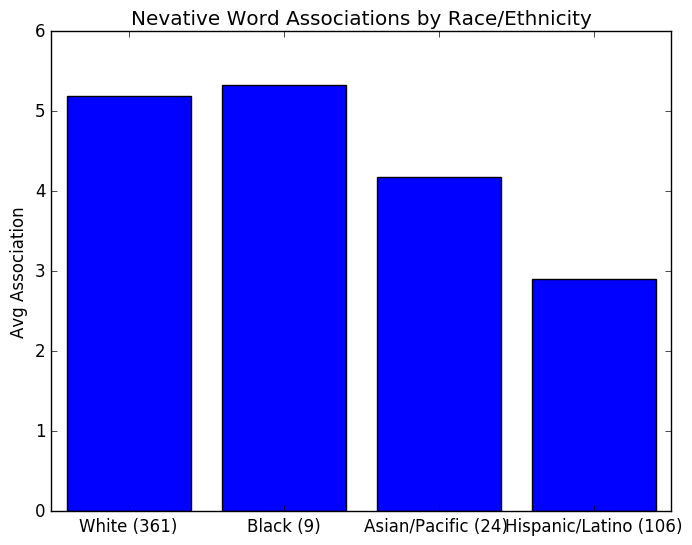
\includegraphics[width=\columnwidth]{images/fig1.png}
\caption{Include some caption that analyzes the graph}
\label{Figure 1}
\end{figure}

\begin{figure}
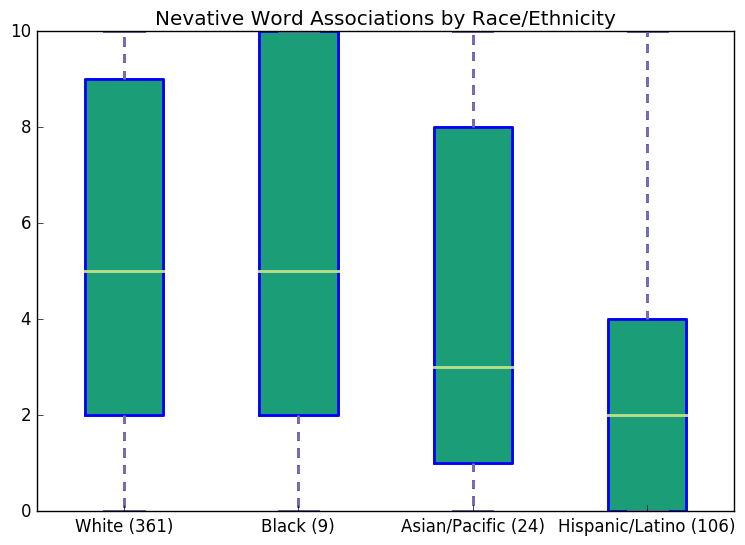
\includegraphics[width=\columnwidth]{images/fig2.png}
\caption{Include some caption that analyzes the box plot}
\label{Figure 2}
\end{figure}

\begin{figure}
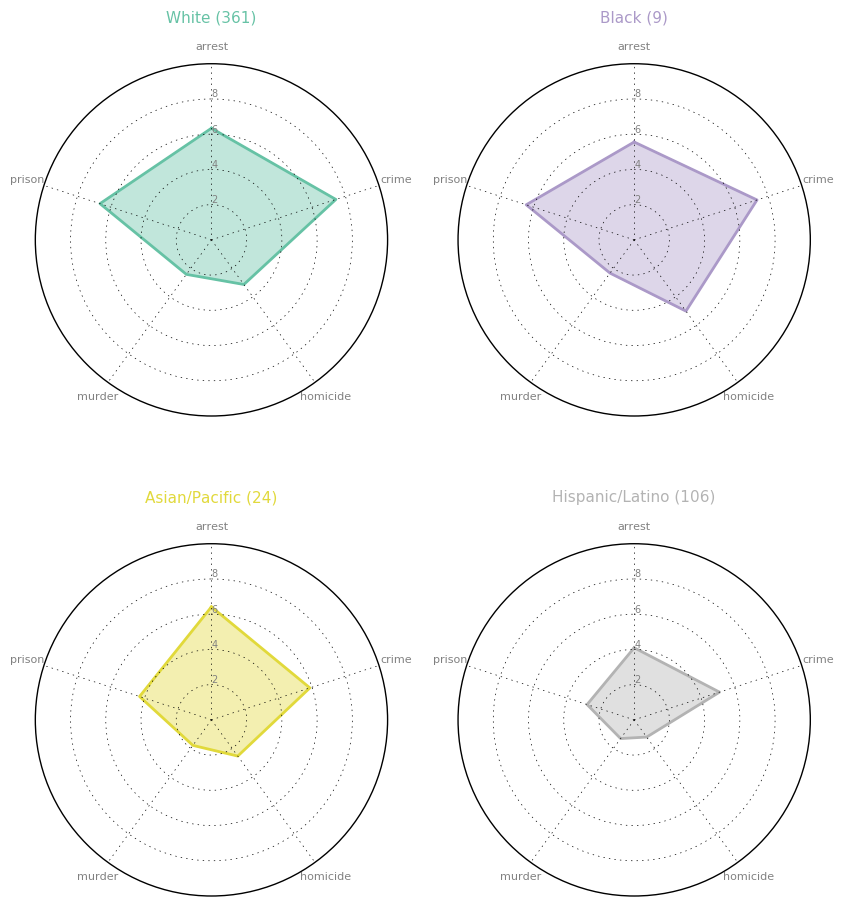
\includegraphics[width=\columnwidth]{images/fig3.png}
\caption{Include some caption that analyzes the charts}
\label{Figure 3}
\end{figure}

\begin{figure}
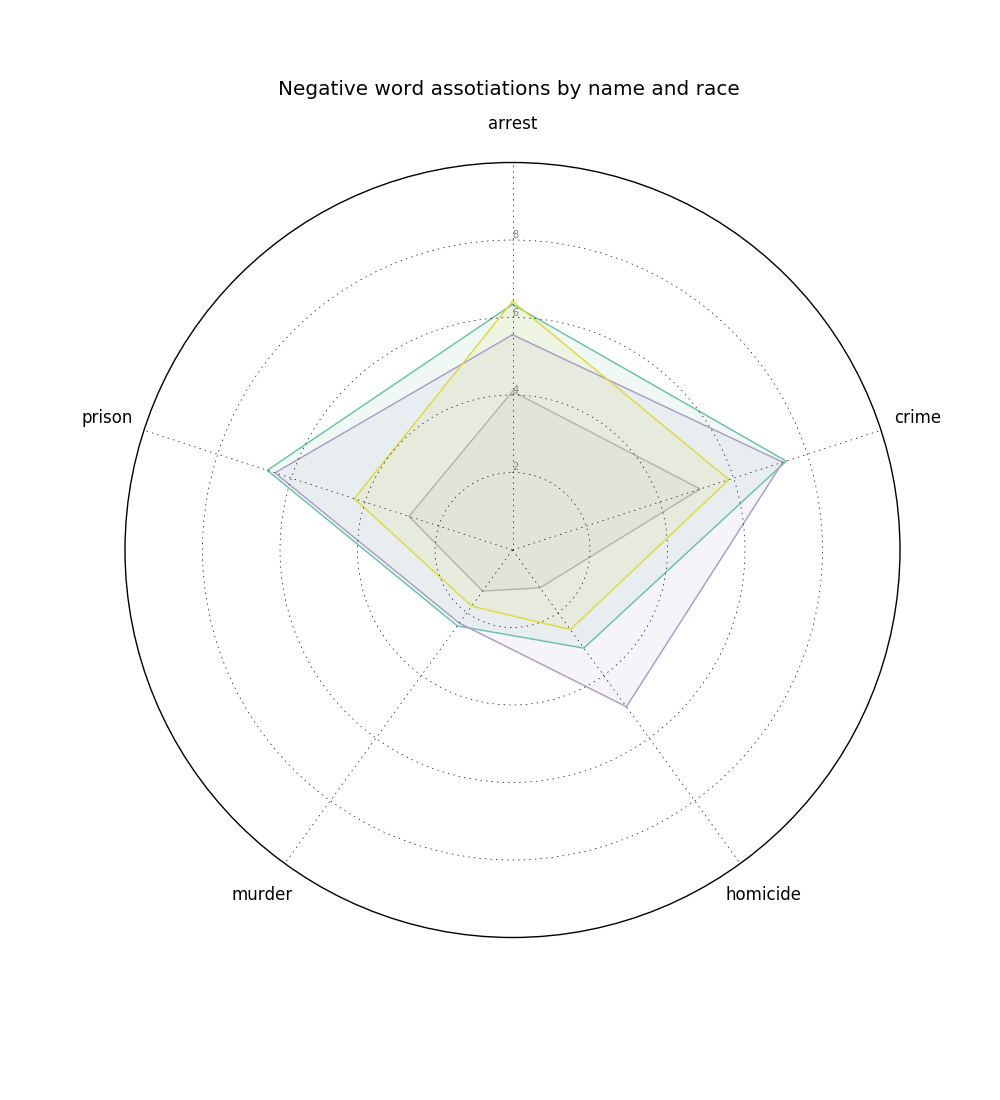
\includegraphics[width=\columnwidth]{images/fig4.png}
\caption{Include some caption that analyzes the chart}
\label{Figure 4}
\end{figure}


\subsection{Discussion}

\section{Conclusion}

In the face of the copious amounts of new issues and problems we find around us when dealing with Big Data, there must be ways that we can hold Big Data and ourselves accountable. In order for Big Data to be the revolutionary force it promises to be, we must find ways to reduce bias and ultimately deal with ethical dilemmas in a proper manner. There are plenty of people around the world trying to solve these problems and progress is certainly being made. As humans, we will never be perfect, but understanding our imperfections and improving on our flaws is definitely a step in the right direction. Is there a way to catch our mistakes that we unwittingly make before we even know that we made them? Multiple cases studies suggest that the answer is a resounding yes: that we can make make algorithms which test for algorithmic bias. Such methods represent the future of Big Data; the idealized future will arrive when we successfully situate it within the broader context of data analysis in general, subjecting it to the same levels of scrutiny as we do for other types of data. We can simultaneously capitalize on Big Data's grand potential while avoiding ethical pitfalls when we successfully allow for transparent analysis; maintain clear, appropriately quantifiable objectives; and include feedback mechanisms that allow us to hone and refine the algorithms to produce objective results. 


\begin{acks}
The authors would like to thank Professor Gregor von Laszewski for providing the opportunity to explore a topic of deep interest.

\end{acks}


\bibliographystyle{ACM-Reference-Format}
\bibliography{report} 

\end{document}
